\documentclass{standalone}
\usepackage{graphicx}	
\usepackage{amssymb, amsmath}
\usepackage{color}

\usepackage{tikz}
\usetikzlibrary{intersections, backgrounds, math}
\usepackage{pgfmath}

\definecolor{light}{RGB}{220, 188, 188}
\definecolor{mid}{RGB}{185, 124, 124}
\definecolor{dark}{RGB}{143, 39, 39}
\definecolor{highlight}{RGB}{180, 31, 180}
\definecolor{light_teal}{RGB}{107, 142, 142}
\definecolor{mid_teal}{RGB}{72, 117, 117}
\definecolor{dark_teal}{RGB}{29, 79, 79}
\definecolor{gray10}{gray}{0.1}
\definecolor{gray20}{gray}{0.2}
\definecolor{gray30}{gray}{0.3}
\definecolor{gray40}{gray}{0.4}
\definecolor{gray60}{gray}{0.6}
\definecolor{gray70}{gray}{0.7}
\definecolor{gray80}{gray}{0.8}
\definecolor{gray90}{gray}{0.9}
\definecolor{gray95}{gray}{0.95}

\begin{document}

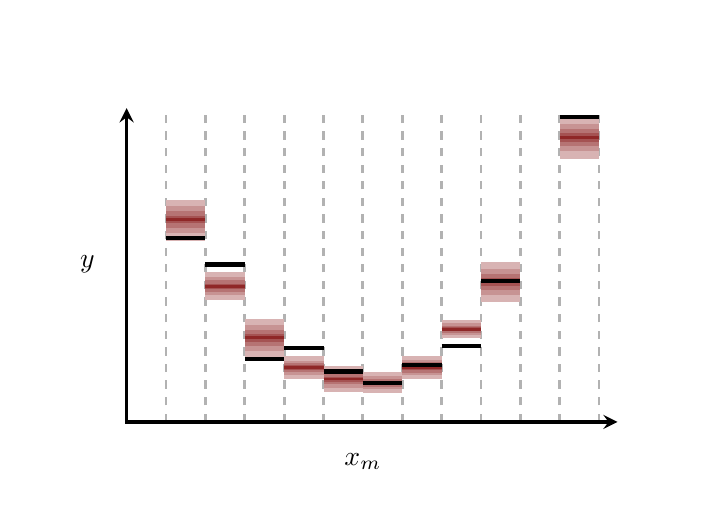
\begin{tikzpicture}[scale=1.0]

  \begin{scope}[shift={(0, 0)}]
    \draw[white] (-4.25, -3) rectangle (4.25, 3);
    
    \foreach \b in {-3.0, -2.5, ..., 3} {
      \draw[gray70, dashed, line width=1] (\b, -2) -- (\b, 2);
    }

    \pgfmathsetmacro{\ys}{0.4};
    \pgfmathsetmacro{\yo}{-1.5};
    
    \pgfmathsetmacro{\prop}{20 + 15 * 1};
    \colorlet{custom}{dark!\prop!white};
    
    \foreach \a/\b/\c/\d  in {-2.500/-2.000/4.510/5.792, 
                              -2.000/-1.500/2.636/3.498, -1.500/-1.000/0.798/2.026,
                              -1.000/-0.500/0.109/0.832, -0.500/0.000/-0.310/0.541, 
                              0.000/0.500/-0.331/0.332, 0.500/1.000/0.109/0.850, 
                              1.000/1.500/1.413/1.990, 1.500/2.000/2.571/3.822, 
                              2.500/3.000/7.109/8.430} {
       \fill[custom] (\a, \ys * \c + \yo) rectangle (\b, \ys * \d + \yo);
    }
    
    \pgfmathsetmacro{\prop}{20 + 15 * 2};
    \colorlet{custom}{dark!\prop!white};
    
    \foreach \a/\b/\c/\d  in {-2.500/-2.000/4.739/5.597, -2.000/-1.500/2.782/3.342, -1.500/-1.000/1.013/1.820, -1.000/-0.500/0.240/0.697, -0.500/0.000/-0.161/0.383, 0.000/0.500/-0.207/0.209, 0.500/1.000/0.234/0.730, 1.000/1.500/1.515/1.897, 1.500/2.000/2.795/3.607, 2.500/3.000/7.354/8.197} {
       \fill[custom] (\a, \ys * \c + \yo) rectangle (\b, \ys * \d + \yo);
    }
    
    \pgfmathsetmacro{\prop}{20 + 15 * 3};
    \colorlet{custom}{dark!\prop!white};
    
    \foreach \a/\b/\c/\d  in {-2.500/-2.000/4.901/5.434, -2.000/-1.500/2.887/3.245, -1.500/-1.000/1.166/1.668, -1.000/-0.500/0.326/0.619, -0.500/0.000/-0.057/0.286, 0.000/0.500/-0.137/0.122, 0.500/1.000/0.318/0.639, 1.000/1.500/1.577/1.804, 1.500/2.000/2.941/3.453, 2.500/3.000/7.501/8.051} {
       \fill[custom] (\a, \ys * \c + \yo) rectangle (\b, \ys * \d + \yo);
    }
    
    \pgfmathsetmacro{\prop}{20 + 15 * 4};
    \colorlet{custom}{dark!\prop!white};
    
    \foreach \a/\b/\c/\d  in {-2.500/-2.000/5.057/5.299, -2.000/-1.500/2.976/3.142, -1.500/-1.000/1.302/1.550, -1.000/-0.500/0.408/0.544, -0.500/0.000/0.032/0.189, 0.000/0.500/-0.069/0.060, 0.500/1.000/0.400/0.557, 1.000/1.500/1.627/1.750, 1.500/2.000/3.073/3.328, 2.500/3.000/7.640/7.923} {
       \fill[custom] (\a, \ys * \c + \yo) rectangle (\b, \ys * \d + \yo);
    }
    
     \foreach \a/\b/\c  in {-2.500/-2.000/5.173, -2.000/-1.500/3.053, -1.500/-1.000/1.422, -1.000/-0.500/0.479, -0.500/0.000/0.112, 0.000/0.500/-0.002, 0.500/1.000/0.481, 1.000/1.500/1.686, 1.500/2.000/3.204, 2.500/3.000/7.782} {
       \draw[dark, line width=1] (\a, \ys * \c + \yo) -- (\b, \ys * \c + \yo);
    }
    
    
    \foreach \l/\r/\m in {-2.500/-2.000/4.591, -2.000/-1.500/3.747, -1.500/-1.000/0.737, -1.000/-0.500/1.097, -0.500/0.000/0.353, 0.000/0.500/-0.020, 0.500/1.000/0.555, 1.000/1.500/1.171, 1.500/2.000/3.226, 2.500/3.000/8.437} {
      \draw[black, line width=1.5] (\l, \ys * \m + \yo) -- (\r, \ys * \m + \yo);
    }
     
    \draw [->, >=stealth, line width=1.25] (-3.00, -2.015) -- +(0, 4);
    \draw [->, >=stealth, line width=1.25] (-3.015, -2.00) -- +(6.25, 0);
    
    \node at (-3.5, 0) { $y$ };
    \node at (0, -2.5) { $x_{m}$ };
  \end{scope}
  
\end{tikzpicture}

\end{document}  